\chapter{Field Models}

	\section{\texttt{PyGeopack}: Python wrapper for the Tsyganenko field models}

		This is a Python module for obtaining field vectors and traces of the Tsygenenko field models. It is a wrapper of a wrapper (see \ref{sectGeopack}). The latest code can be viewed and downloaded from here: \href{https://github.com/mattkjames7/PyGeopack}{https://github.com/mattkjames7/PyGeopack}.

		\subsection{Installation}

			The easiest way to install \texttt{PyGeopack} is using \texttt{pip}, e.g.:
			\begin{minted}{bash}
pip3 install PyGeopack --user
			\end{minted}
			for other installation methods, see the GitHub repo.

			At this point, it \textit{may} just work if you were to try to import it, but there's a reasonably good chance that the C++/Fortran code will need to be recompiled, in which case we need to ensure that there are compilers available to do this (see section \rec{sectSetup}). 

			One of the features of PyGeopack is that it can easily package together all of the geomagnetic/solar wind parameters that the models use so that when you request a trace or a field vector for a specific date and time, it will automatically try to find the appropriate parameters. This isn't strictly necessary for the models to work, as they will default to some fairly average parameters and they can be overridden manually. In order to be able to use this functionality, this module and the submodules which it relies on to collect the relevant data need to know where they can store the parameters. This means exporting a few environment variables (e.g. in \texttt{$\sim$/.bashrc}):
			\begin{minted}{bash}
export KPDATA_PATH=/path/to/kp
export OMNIDATA_PATH=/path/to/omni
export GEOPACK_PATH=/path/to/geopack/data				
			\end{minted}
			which are set as follows for me on SPECTRE:
			\begin{minted}{bash}
export KPDATA_PATH="/data/sol-ionosphere/mkj13/Kp"
export OMNIDATA_PATH="/data/sol-ionosphere/mkj13/OMNI"
export GEOPACK_PATH="/data/sol-ionosphere/mkj13/Geopack"			
			\end{minted}	
			
			Once that is done, it should work...
		
		\subsection{Usage}

			The first time this is imported, there is a good chance that it will attempt to recompile itself. There will be a lot of messages on the screen, but it should finish successfully. If it fails, double check that you have the required compilers installed, raise an issue on the GitHub page if the problem persists.

			If you would lke the latest model parameters, run the following:
			\begin{minted}{python}
import PyGeopack as gp
gp.Params.UpdateParameters(SkipWParameters=True)
			\end{minted}
			This may take a little time, depending on how much data it needs to download. It will take all of the data and compile it into one binary file $\sim$350 MiB in size, once this is done, it should be relatively quick loading the data into memory.

			The model field vectors can be returned using the \texttt{ModelField} function:
			\begin{minted}{python}
Bx,By,Bz = gp.ModelField(x,y,z,Date,ut,Model='T96',CoordIn='GSM',**kwargs)
			\end{minted}
			where \texttt{x}, \texttt{y} and \texttt{z} can be scalars or arrays of position, in units of Earth radii and in the coordinate system defined by the \texttt{CoordIn} keyword (\texttt{'GSE'|'GSM'|'SM'}). \texttt{Date} can be an array or scalar of date(s) in the format yyyymmdd, while \texttt{ut} is in hours from the start of the day. The models currently available are \texttt{'T89'}, \texttt{'T96'}, \texttt{'T01'} and  \texttt{'TS05'}.

			Traces are simple to produce and can be done a single trace at a time, or in batches, e.g.:
			\begin{minted}{python}
import numpy as np

#define a few starting positions for the traces
x = np.array([2.0,4.0,6.0,8.0])
y = np.array([0.0,0.0,0.0,0.0])
z = np.array([0.0,0.0,0.0,0.0])

#run the traces, return TraceField object
T = gp.TraceField(x,y,z,20221222,16.0)

#plot field traces
ax = T.PlotRhoZ()
			\end{minted}
			which should produce a plot similar to figure \ref{figGeopackTrace}.

			\begin{figure}
				\centering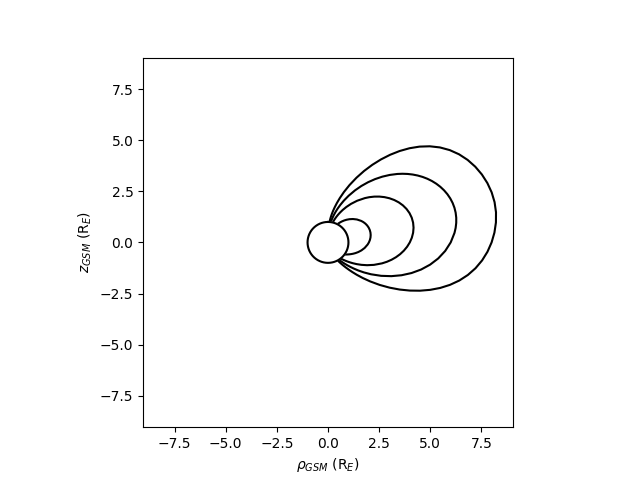
\includegraphics[width=\textwidth]{figures/ch03_geopacktrace.png}
				\caption{Example of field tracing using \texttt{PyGeopack}.
					\label{figGeopackTrace}}
			\end{figure}

			For more information on the keyword arguments please see the \href{https://github.com/mattkjames7/PyGeopack/blob/master/README.md}{readme}.

	\section{\texttt{geopack}: C++ wrapper for Tsyganenko field models}

		\label{sectGeopack}

	\section{\texttt{libinternalfield}: C++ spherical harmonic model code}

	\section{\texttt{vsmodel}: Python based Volland-Stern electric field model for Earth}

	\section{\texttt{JupiterMag}: Python wrapper for Jovian field models}

	\section{\texttt{libjupitermag}: C++ library for field tracing in Jupiter's magnetosphere}

	\section{\texttt{con2020}: Python implementation of Jupiter's magnetodisc model}

	\section{\texttt{libcon2020}: C++ implementation of Jupiter's magnetodisc model}

	\section{\texttt{jrm33}: The JRM33 model in Python}

	\section{\texttt{jrm09}: The JRM09 model in Python}

	\section{\texttt{vip4model}: The VIP4 model in Python}
	